% Beginning code for all standard physics latex documents

%Created on: May 8, 2014    Edited by: Wesley Kyle
%Edited on:	May 12, 2016	Edited by: P. Gimby - cleaned up the code to remove unneeded packages
%Edited on:	May 13, 2016	Edited by: P. Gimby - collected a few more packages used in 325.
%Edited on:	May 16, 2016	Edited by: P. Gimby - fixed page numbering error.
%Edited on: May 20, 2016	Edited by: Alex Shook - Added packages for 497

\documentclass[justified]{tufte-book}
\usepackage{graphicx} % allow embedded images
\setkeys{Gin}{width=\linewidth,totalheight=\textheight,keepaspectratio}
\usepackage{amsmath}  % extended mathematics
\usepackage{bm}  % bold font in math mode
\usepackage{longtable} %lets long tables flow into multiple pages instead of running off the page or having to break tables up manually
\usepackage{booktabs} % book-quality tables
\usepackage{units}    % non-stacked fractions and better unit spacing
\usepackage{multicol} % multiple column layout facilities
\usepackage{tikz} %for drawing nice pictures
\usepackage{indentfirst} % makes first line of each new section be indented
\usepackage{enumitem} % extended options for the enumerate environment
\usepackage{soul} % gives more typestting options like spacing, underline, and strike-through
\usepackage{marvosym} %extra symbols package
\usepackage{multirow} % for special table controls
\usepackage[singlelinecheck=false]{caption} % allow captions w/o figure number
\captionsetup{compatibility=false} % corrects in issue with the caption package
\usepackage{float} % allows for contorl over position of figures and tables
\allowdisplaybreaks % allows equations to span two pages if needed
\usepackage{mathrsfs} % fancy math symbols
\usepackage{multirow} % for special table controls
\usetikzlibrary{arrows,shapes,snakes,calc,patterns,3d} % addon to tikz
\usetikzlibrary{circuits.ee.IEC} % addon to tikz
\usepackage{pgfplots} % package for making plots of functions
\usepackage{gensymb} % symbols i,e. degrees
\usetikzlibrary{decorations.pathmorphing} % to draw the springs
\tikzset{circuit declare symbol = ac source}
\tikzset{set ac source graphic = ac source IEC graphic}
\usepackage{changepage} % allows for full page environment
\usepackage{comment} % allows comment tags for large sections

% define new page style that puts page numbers in the middle
%\begin{comment}
\fancypagestyle{custom}{
\fancyhf{} % clear all header and footer fields
\fancyheadoffset{0pt}
\fancyfootoffset{0pt}
\fancyfoot[C]{\thepage}
\renewcommand{\headrulewidth}{0pt}
\renewcommand{\footrulewidth}{0pt}}
\pagestyle{custom}
%\end{comment}

%below creates a new circuit symbol for AC sources
\tikzset{
         ac source IEC graphic/.style=
          {
           transform shape,
           circuit symbol lines,
           circuit symbol size = width 3 height 3,
           shape=generic circle IEC,
           /pgf/generic circle IEC/before background=
            {
             \pgftransformresetnontranslations
             \pgfpathmoveto{\pgfpoint{-0.8\tikzcircuitssizeunit}{0\tikzcircuitssizeunit}}
             \pgfpathsine{\pgfpoint{0.4\tikzcircuitssizeunit}{0.4\tikzcircuitssizeunit}}
             \pgfpathcosine{\pgfpoint{0.4\tikzcircuitssizeunit}{-0.4\tikzcircuitssizeunit}}
             \pgfpathsine{\pgfpoint{0.4\tikzcircuitssizeunit}{-0.4\tikzcircuitssizeunit}}
             \pgfpathcosine{\pgfpoint{0.4\tikzcircuitssizeunit}{0.4\tikzcircuitssizeunit}}
             \pgfusepathqstroke
            }
          }
        }
% end of circuit symbol
%\begin{document}
%%%end individual beginning code/,$d


%  \begin{titlepage}
%    \vspace*{\fill}
%    \begin{center}
%      \huge{{\bf TITLE1}}\\[0.4cm]
%      \huge{TITLE2}\\[0.4cm]
%      \LARGE{Laboratory Manual}\\[0.4cm]
%      \large{SEASON YEAR}
%    \end{center}
%    \vspace*{\fill}
%  \end{titlepage}
%\maketitle

%\begin{spacing}{0.5}
%\tableofcontents
%\end{spacing}

%NEW PHYS 497 PACKAGES AND COMMANDS

%Subcaption package: Allows subfigures to be placed side by side, and labeled with individual captions (Added June 1, 2016)
\usepackage{subcaption}

%Array package: Allows for addiation specifications in arrays (Added May 6, 2016)
\usepackage{array}

%newcolumntype: Allows one to specify a fixed column width (Added May 6, 2016)
\newcolumntype{L}[1]{>{\raggedright\let\newline\\\arraybackslash\hspace{0pt}}m{#1}}
\newcolumntype{C}[1]{>{\centering\let\newline\\\arraybackslash\hspace{0pt}}m{#1}}
\newcolumntype{R}[1]{>{\raggedleft\let\newline\\\arraybackslash\hspace{0pt}}m{#1}}

%circuits.logic.US, circuits.logic.IEC: For drawing logic gates in Tikz (Added May 6, 2016) 
\usetikzlibrary{circuits.logic.US,circuits.logic.IEC}

\newcommand{\PGT}{ %PGT: positive going transition
\begin{tikzpicture}
\draw[-angle 60] (0,0) -- (0,5pt);
\draw (0,5pt) -- (0,6pt) -- (5pt,6pt);
\draw (-5pt,0) -- (0,0);
\end{tikzpicture}
}





%TEST
\usepackage{geometry}
\pagestyle{fancy}

%\usepackage[caption=false]{subfig}

%\makeatletter
%\renewenvironment{figure}[1][htbp]{%
%  \@tufte@orig@float{figure}[#1]%
%}{%
%  \@tufte@orig@endfloat
%}

%\renewenvironment{table}[1][htbp]{%
%  \@tufte@orig@float{table}[#1]%
%}{%
%  \@tufte@orig@endfloat
%}
%\makeatother

% use instead of subfigure
\makeatletter
\newenvironment{multifigure}[1][htbp]{%
  \@tufte@orig@float{figure}[#1]%
}{%
  \@tufte@orig@endfloat
}
\makeatother

\makeatletter
\newenvironment{mainfigure}[1][htbp]{%
\@tufte@orig@float{figure}[#1]
\begin{adjustwidth}{}{-153pt}}
{\end{adjustwidth}\@tufte@orig@endfloat}%
\makeatother

\makeatletter
\newenvironment{maintable}[1][htbp]{%
\@tufte@orig@float{table}[#1]
\begin{adjustwidth}{}{-153pt}}
{\end{adjustwidth}\@tufte@orig@endfloat}%
\makeatother

%%%% Labatorial Cross-over labs need this code. This should be temporary PG Dec 7, 2016

\newcounter{questioncounter}
\setcounter{questioncounter}{0}
\newcounter{checkpointcounter}
\setcounter{checkpointcounter}{0}
\newcounter{figurecounter}
\setcounter{figurecounter}{0}
%%%%%%%%%%%%%%%%%%%%%%%%%%%%%%%%%%%%%%%%%%%%%%%%%%%%%%%

\newcommand{\checkpoint}{
 \fbox{\begin{minipage}{0.2\textwidth}
 %\includegraphics[width=0.5\textwidth]{stop}
 \end{minipage}
 \begin{minipage}{1.0\textwidth}
 {\bf CHECKPOINT \addtocounter{checkpointcounter}{1} \arabic{checkpointcounter}: Before moving on to the next part, have your TA check the results you obtained so far.}
 \end{minipage}}}

%%% end labatorial cross-over code.

% New environment for placing figure captions under the figure
%\makeatletter
%\newenvironment{mainfigure}{\textwidth}[1][htbp]{%
%\@tufte@orig@float{figure}[#1]%
%}{%
%\@tufte@orig@endfloat
%}
%\makeatother

\begin{document}
%%%%%%%%%%%%%%%%%%%%%%%%%%%%%%%%%%%%%%%%%%%%%
%
% RLC Resonant Circuits
%
%%%%%%%%%%%%%%%%%%%%%%%%%%%%%%%%%%%%%%%%%%%%%


\setcounter{chapter}{5}
\setcounter{equation}{0}
\setcounter{table}{0}
\setcounter{figure}{0}
\chapter{RLC Resonant Circuits}

\section{Equipment}

% first column
\begin{minipage}[t]{0.6\textwidth}
\begin{itemize}[noitemsep]
\item Series and parallel RLC circuit board
\item B \& K 3011 function generator
\item set of connecting leads (2)
\end{itemize}
\end{minipage}
%second column
\begin{minipage}[t]{0.35\textwidth}
\begin{itemize}[noitemsep]
\item Oscilloscope
\end{itemize}
\end{minipage}

\begin{marginfigure}[+1in]
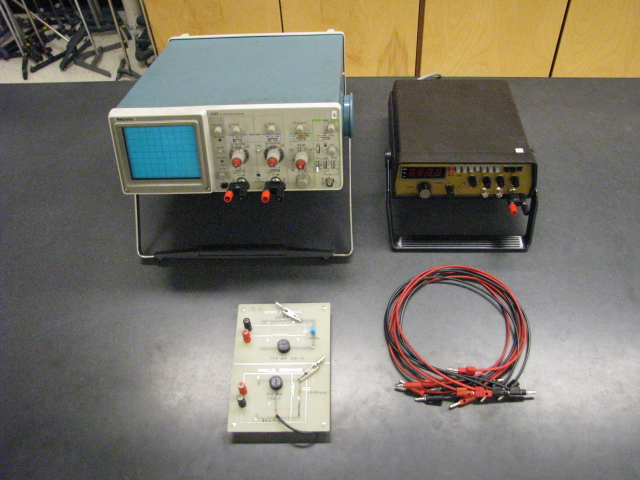
\includegraphics{/usr/local/master/labs/physics397-FA2016/RLC-Resonant-Circuits/RLC-Resonant-Circuits-Setup.jpg}
\caption{A photograph of the experimental setup.}
\label{fig:RLsetup}
\end{marginfigure}

\section{Preparation}
Review the theory of RLC resonant circuits. Study the principles of AC signals and their application to resistors, inductors, and capacitors. 

\section{Purpose}
To learn to construct series and parallel RLC circuits and be able to calculate through theory and measurements, the amplitude resonance and the phase resonance of them. Lastly, to learn to measure phase resonance via x-y oscilloscope measurements.

\section{Theory}
The current delivered to homes and factories is an oscillating function of time. This is called {\bf alternating current}, or {\bf AC}. All the appliances connected to ordinary outlets in homes therefore involve circuits with oscillating currents. Furthermore, electronic devices, such as radio transmitters and receivers, involve a variety of circuits with oscillating currents of high frequency. Many of these circuits have natural frequencies of oscillation. Such circuits exhibit the phenomenon of {\bf resonance} when the natural frequency matches the frequency of a signal applied to the circuit. For instance, the tuning of a radio relies on an oscillating circuit whose frequency of oscillation is adjusted by means of a variable capacitor so that it matches the frequency of the radio signal.

A common circuit known as the {\bf RLC circuit} exhibits the phenomenon of resonance. It is named RLC because it includes a resistor, capacitor, and inductor. There are two different kinds of RLC circuit. A {\bf series RLC circuit} is explained in section I and the {\bf parallel RLC circuit} is explained in section II.

\section{I - Series RLC Circuits}
The series RLC circuit used in this experiment is shown in Figure \ref{fig:rc1}. The values of resistance, $R_r$, capacitance, C, and inductance, L, are written on the components themselves. The total resistance of the circuit, R, is the sum of the resistances of the resistor, $R_r$, and the inductor, $R_L$.

\begin{marginfigure}
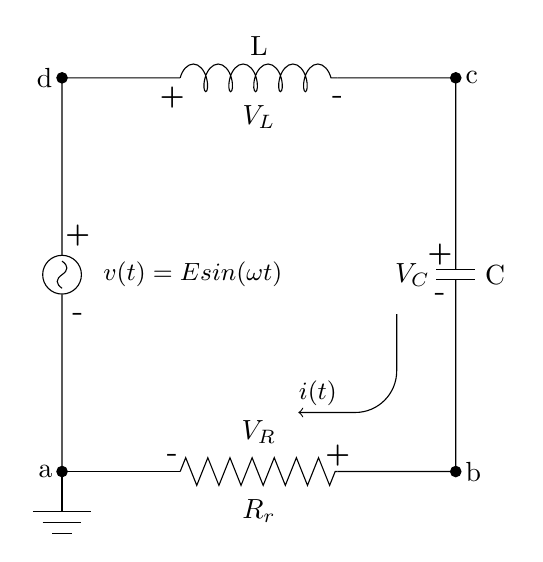
\begin{tikzpicture}[circuit ee IEC]
%circuit
\draw(0,0)to [ac source](0,5)--(1.5,5);
\draw[decorate,decoration={coil,segment length=9,amplitude=5}](1.5,5)--(3.5,5);
\draw(3.5,5)--(5,5)to[capacitor](5,0)--(3.5,0);
\draw[decorate,decoration={zigzag,segment length=8,amplitude=5}](1.5,0)--(3.5,0);
\draw(1.5,0)--(0,0)--(0,-.5);
\node[ground,rotate=-90,scale=1.5]at(0,-.65){}; %ground
%labels
\node[] at(4.8,2.75){{\bf +}};
\node[] at(1.4,4.75){{\bf +}};
\node[] at(3.5,.2){{\bf +}};
\node[] at(.2,3){{\bf +}};
\node[font=\large] at(4.8,2.25){-};
\node[font=\large] at(3.5,4.75){-};
\node[font=\large] at(1.4,.2){-};
\node[font=\large] at(.2,2){-};
\node[shape=circle,draw=black,fill=black,scale=.4] at (0,0){};
\node[shape=circle,draw=black,fill=black,scale=.4] at (5,0){};
\node[shape=circle,draw=black,fill=black,scale=.4] at (5,5){};
\node[shape=circle,draw=black,fill=black,scale=.4] at (0,5){};
\node[right,font=\small] at(.4,2.5){$v(t)=Esin(\omega t)$};
\node[left] at(0,0){a};
\node[right] at(5,0){b};
\node[right] at(5,5){c};
\node[left] at(0,5){d};
\node[] at(2.5,5.4){L};
\node[] at(2.5,4.5){$V_L$};
\node[] at(5.5,2.5){C};
\node[] at(4.45,2.5){$V_C$};
\node[] at(2.5,-.5){$R_r$};
\node[] at(2.5,.5){$V_R$};
\draw[rounded corners=15,->](4.25,2)--(4.25,.75)--(3,.75);
\node[font=\small] at(3.25,1){$i(t)$};
\end{tikzpicture}
\caption{Series RLC circuit.}
\label{fig:rc1}
\end{marginfigure}

Assume that the internal resistance of the function generator can be ignored and choose the input signal to be $v(t)=Esin(\omega t)$, where E is the maximum emf. The emf acts as a driving force that moves the charge in the circuit. An application of {\bf Kirchoff's voltage law} gives

\begin{equation}
\sum V=0=V_L+V_C+V_R-Esin(\omega t)
\label{equ:rc1}
\end{equation}

\noindent where

\begin{equation}
V_C=\dfrac{1}{C}\int i\cdot dt
\label{equ:rc2}
\end{equation}

\begin{equation}
V_L=L\dfrac{di}{dt}
\label{equ:rc3}
\end{equation}

\noindent and

\begin{equation}
V_R=iR
\label{equ:rc4}
\end{equation}

\noindent are the AC voltages across each component.

Substituting Equations \ref{equ:rc2}, \ref{equ:rc3}, and \ref{equ:rc4} into Equation \ref{equ:rc1} and rearranging gives the expression

\begin{equation}
Esin(\omega t)=\dfrac{1}{C}\int i\cdot dt +L\dfrac{di}{dt}+iR
\label{equ:rc5}
\end{equation}

Differentiating both sides with respect to time, $t$, to remove the integral, yields the differential equation


\begin{equation}
E\omega cos(\omega t)=\dfrac{i}{C}+L\dfrac{d^2i}{dt^2}+R\dfrac{di}{dt}
\label{equ:rc6}
\end{equation}

\noindent The steady state solution of this equation is


\begin{equation}
i(t)=\dfrac{E}{\sqrt{R^2+\left(\omega L-\dfrac{1}{\omega C}\right)}}\cdot sin(\omega t-\phi)
\label{equ:rc7}
\end{equation}

\noindent where


\begin{equation}
\phi=tan^{-1}\left[\dfrac{1}{R}\left(\omega L-\dfrac{1}{\omega C}\right)\right]
\label{equ:rc8}
\end{equation}

The {\bf angular frequency}, $\omega$, is $2\pi f$, where $f$ is the frequency in cycles per second or Hertz (Hz). Equations \ref{equ:rc7} and \ref{equ:rc8} imply that the current flowing in a series RLC circuit is a sine wave with an amplitude that changes with frequency and a phase difference from the signal generator that also changes with frequency. So the behaviour of the circuit strongly depends on the frequency of the applied voltage.

For Equation \ref{equ:rc7}, the current, $i(t)$, becomes an extremum when $\omega^2 = 1/LC$. The condition when the amplitude of $i(t)$ is an extremum is known as {\bf amplitude resonance}. For series RLC circuits, the extremum turns out to be a {\bf maximum}. Thus, at amplitude resonance the current flowing in the circuit has maximum amplitude. At all other frequencies, the current flowing in the circuit is smaller. This property makes the series RLC circuit useful in filters where a response at one frequency is preferred over all other frequencies. This is what happens in radio receivers when one station is selected. The frequency corresponding to the carrier of that station is chosen to be the amplitude resonant frequency.

When $\omega^2 = 1/LC$, Equation \ref{equ:rc8} implies that $\phi = 0$. The condition when $\phi  = 0$ is called {\bf phase resonance}. At phase resonance, the signals at points {\bf d} and {\bf b} in Figure \ref{fig:rc1} are in phase. So there is no phase difference between the applied voltage and the current. In series RLC circuits, amplitude and phase resonance both happen at the {\bf same frequency}. In other types of circuits this is not necessarily true.

\begin{marginfigure}
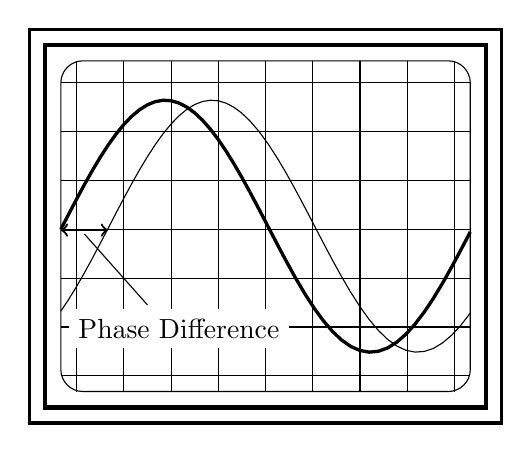
\begin{tikzpicture}
%frame of oscilloscope
\draw[very thick](0,0)rectangle(6,5);
\draw[ultra thick](.2,.2)rectangle(5.8,4.8);
\draw[rounded corners=8](.4,.4)rectangle(5.6,4.6);
%grid on screen
\foreach \y in {0,...,6}
{
\draw[thin](.4,.6+\y*.62)--(5.6,.6+\y*.62);
}
\foreach \x in {0,...,8}
{
\draw[thin](.6+\x*.6,.4)--(.6+\x*.6,4.6);
}
\draw[very thick,domain=.4:2.8] plot (\x, {1.6*sin(\x*69-29)+2.5}); %function
\draw[very thick,domain=2.8:5.6] plot (\x, {1.6*sin(\x*69-29)+2.5}); %function
\draw[thin,domain=.4:2.8] plot (\x, {1.6*sin(\x*69-70)+2.5}); %phase shifted function
\draw[thin,domain=2.8:5.6] plot (\x, {1.6*sin(\x*69-70)+2.5}); %phase shifted function
%labels
\node[shape=rectangle,fill=white, draw=white, right] at (.5,1.2){Phase Difference};
\draw[thick,<->](.4,2.45)--(1,2.45);
\draw[thin](1.5,1.5)--(.7,2.4);
\end{tikzpicture}
\caption{An illustration of phase difference.}
\label{fig:rc2}
\end{marginfigure}

The oscilloscope screen in Figure \ref{fig:rc2} shows two signals that are out of phase. A phase difference between two waveforms is usually reported as an angle. Since horizontal distances on an oscilloscope are in terms of time, a conversion from time to angle has to be made. This is done by noting that the time for a full cycle is 360$^{\circ}$, so the actual phase difference as an angle is found by determining it as a fraction of one cycle and multiplying by 360$^{\circ}$.

To measure a phase difference between two sine waves necessarily implies that they have the same frequency. The phase between two sine waves of different frequency is not constant. Also, notice that the two sinusoidal waveforms depicted in Figure 2 have the same amplitude. This is deliberate. An accurate phase measurement can only made on an oscilloscope when the amplitudes of the signals are the same. Since in general, it is unlikely that any two signals have the same amplitude, a special control is available on the oscilloscope to shift amplitudes without requiring a change to the input signal. This control is called the {\bf vertical calibration} adjustment. To make two signals have the same displayed amplitude simply modify the vertical calibration of one channel. After the phase measurement is completed, remember to return the vertical calibration setting back to normal, otherwise further vertical measurements will be incorrect.

When $i(t)$ becomes an extremum, the input frequency matches the {\bf natural frequency} of the circuit. This is manifested as a voltage extremum on the oscilloscope screen. Thus, when searching for frequencies at which $i(t)$ becomes an extremum, look for frequencies corresponding to a voltage extremum on the oscilloscope screen. The reason for voltage measurements rather than current measurements is due to the fact that the oscilloscope only displays voltages. Moreover, the signal at point {\bf b} is the voltage across the resistor, which is directly proportional to the current by Ohm's law.

\section{II - Parallel RLC Circuits}
The parallel RLC circuit used in this experiment is depicted in Figure \ref{fig:rc3}. The values of resistance, $R_r$, capacitance, C, and inductance, L, are written on the components themselves. Again, the total resistance, R, of the circuit is the sum of the resistances of the resistor, $R_r$, and the inductor, $R_L$.

Again, ignore the internal resistance of the function generator and choose the input signal to have the form $v(t)=Esin(\omega t)$, where E is the maximum emf. This emf acts as a driving force that moves the charge in the circuit. However, in parallel circuits, the behavior of the circuit is given by two simultaneous equations. This is due to the fact that the positions of the inductor and the capacitor are in parallel to each other, thus, the input current splits. Let $i_1(t)$ be the current in the inductive branch and $i_2(t)$ be the current in the capacitive branch. Then {\bf Kirchoff's current law} yields

\begin{marginfigure}
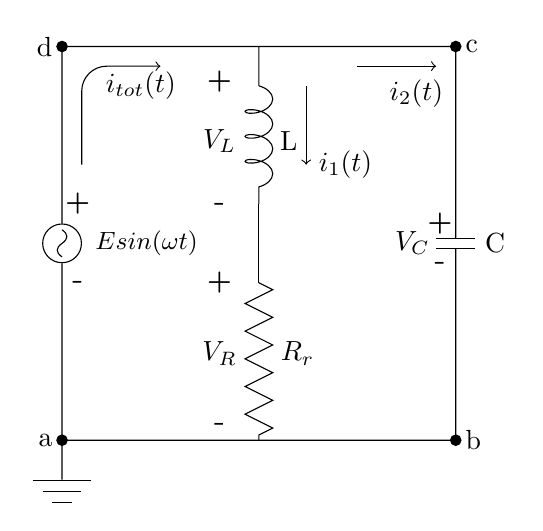
\begin{tikzpicture}[circuit ee IEC]
%circuit
\draw(0,0)to [ac source](0,5)--(2.5,5)--(2.5,4.5);
\draw[decorate,decoration={coil,segment length=9,amplitude=5}](2.5,4.5)--(2.5,3); %inductor
\draw(2.5,5)--(5,5)to[capacitor](5,0)--(0,0)--(0,-.5);
\draw(2.5,2)--(2.5,3);
\draw[decorate,decoration={zigzag,segment length=10,amplitude=5}](2.5,2)--(2.5,0); %resistor
\node[ground,rotate=-90,scale=1.5]at(0,-.65){}; %ground
%labels
\node[] at(4.8,2.75){{\bf +}};
\node[] at(2,4.55){{\bf +}};
\node[] at(2,2){{\bf +}};
\node[] at(.2,3){{\bf +}};
\node[font=\large] at(4.8,2.25){-};
\node[font=\large] at(2,3){-};
\node[font=\large] at(2,.2){-};
\node[font=\large] at(.2,2){-};
\node[shape=circle,draw=black,fill=black,scale=.4] at (0,0){};
\node[shape=circle,draw=black,fill=black,scale=.4] at (5,0){};
\node[shape=circle,draw=black,fill=black,scale=.4] at (5,5){};
\node[shape=circle,draw=black,fill=black,scale=.4] at (0,5){};
\node[left] at(0,0){a};
\node[right] at(5,0){b};
\node[right] at(5,5){c};
\node[left] at(0,5){d};
\node[] at(5.5,2.5){C};
\node[] at(4.45,2.5){$V_C$};
\node[] at(2.99,1.1){$R_r$};
\node[] at(2.,1.1){$V_R$};
\node[] at(2.88,3.8){L};
\node[] at(2.,3.8){$V_L$};
\node[right,font=\small] at(.3,2.5){$Esin(\omega t)$}; %AC source
\draw[rounded corners=9,->](.25,3.5)--(.25,4.75)--(1.25,4.75); %i_tot
\draw[->](3.75,4.75)--(4.75,4.75);
\draw[->](3.1,4.5)--(3.1,3.5);
\node[]at(4.5,4.4){$i_2(t)$}; %i2
\node[]at(3.6,3.5){$i_1(t)$}; %i1
\node[]at(1,4.5){$i_{tot}(t)$};
\end{tikzpicture}
\caption{Parallel RLC circuit.}
\label{fig:rc3}
\end{marginfigure}

\begin{equation}
i_{tot}(t)=i_1(t)+i_2(t)
\label{equ:rc9}
\end{equation}

Furthermore, {\bf Kirchoff's voltage law} gives the equations

\begin{equation}
L\dfrac{di_1}{dt}+Ri_1=Esin(\omega t)
\label{equ:rc10}
\end{equation}

\noindent and

\begin{equation}
\dfrac{i_2}{C}=E\omega cos(\omega t)
\label{equ:rc11}
\end{equation}

These equations have the solution

\begin{equation}
i_{tot}(t)=E\cdot\sqrt{\dfrac{(1-\omega^2LC)^2+(\omega RC)^2}{R^2+(\omega L)^2}}\cdot sin(\omega t+\phi)
\label{equ:rc12}
\end{equation}

\noindent where

\begin{equation}
\phi=tan^{-1}\left[\omega RC+\dfrac{\omega^3L^2C}{R}-\dfrac{\omega L}{R}\right]
\label{equ:rc13}
\end{equation}

In the case of the parallel RLC circuit, the amplitude and the phase resonances do occur at {\bf different frequencies}. For the amplitude resonance frequency, $\omega_A$, Equation \ref{equ:rc12} implies that

\begin{equation}
\omega_A^2=\dfrac{1}{LC}\sqrt{1+\dfrac{2R^2C}{L}}-\dfrac{R^2}{L^2}
\label{equ:rc14}
\end{equation}

\noindent whereas, for the phase resonance frequency, $\omega_P$, Equation \ref{equ:rc13} yields

\begin{equation}
\omega_P^2=\dfrac{1}{LC}-\dfrac{R^2}{L^2}
\label{equ:rc15}
\end{equation}

This experiment examines the resonance phenomena of RLC circuits. The circuits to be examined are shown in Figures \ref{fig:rc1} and \ref{fig:rc3}. The input frequency to the circuit is varied to determine at what frequencies resonances occur. Then, the experimental values obtained can be compared with the theoretical values to assess the validity of the resonance theory.

\section{Experimental Procedure} 
\begin{enumerate}
\item Inspect the function generator and the dual channel oscilloscope. Make sure that the function generator is set to a sine wave output. Also, set the scope to show both channels on the screen simultaneously as this will be needed to verify the phase resonance of the circuits.

\item Before proceeding further, calculate the theoretical amplitude and phase resonant frequencies for  both the series and parallel RLC circuits using the component values displayed on the circuit boards. This will help the experimental search for resonance frequencies.

\item For the {\bf series RLC circuit}, setup the experiment as in Figure \ref{fig:rc4}. Connect both the function generator and channel 1 of the oscilloscope between {\bf d} and {\bf a}, the input pins. Thus the trace on channel 1 will represent the input signal from the function generator. Connect channel 2 of the oscilloscope between {\bf b} and {\bf a}. The channel 2 trace will then be directly proportional to the current going through the circuit.

On the circuit board there is a red and a black connection terminal. When connecting the function generator and the dual channel oscilloscope onto the circuit board, the common ground on the circuit board is the {\bf RED} terminal, while the common ground on the instruments is the black terminal. The reason for this is that the resistor voltage needs to be measured so the oscilloscope ground has to be connected to point {\bf a}.

\begin{figure}
\begin{tikzpicture}[circuit ee IEC]
\node at (0,5){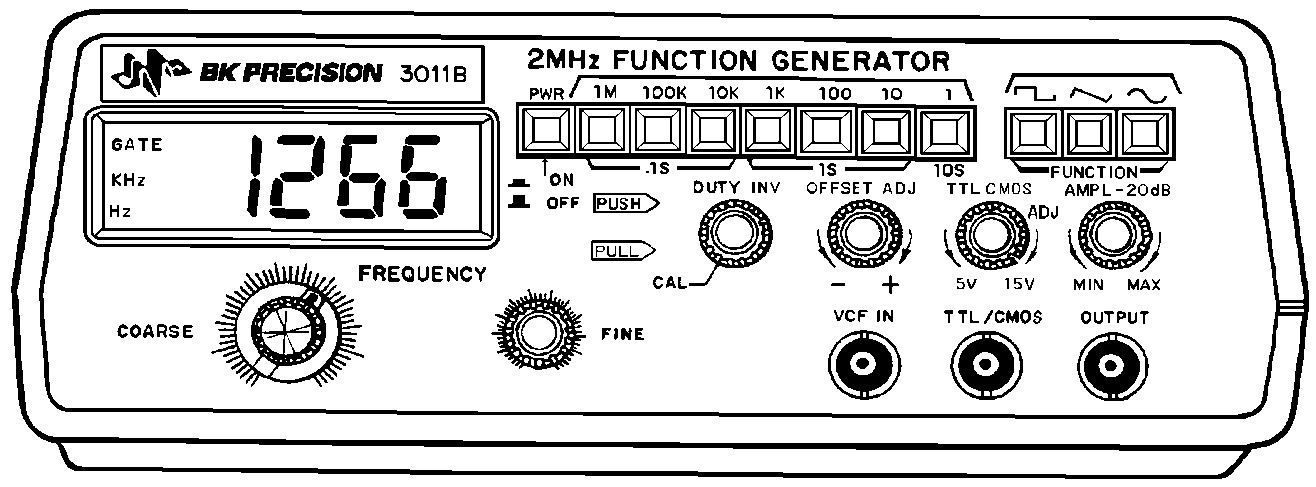
\includegraphics[width=110pt]{/usr/local/master/labs/physics397-FA2016/RLC-Resonant-Circuits/RLC-Resonant-Circuits-func-gen.png}}; %function generator
\draw[thick](1,4.2)rectangle(1.5,4.4);
\node[shape=circle,draw=black,fill=black,scale=.7] at(1.0,4.3){};
\node[shape=circle,draw=black,fill=black,scale=.7] at(1.5,4.3){};
\node at (0,2){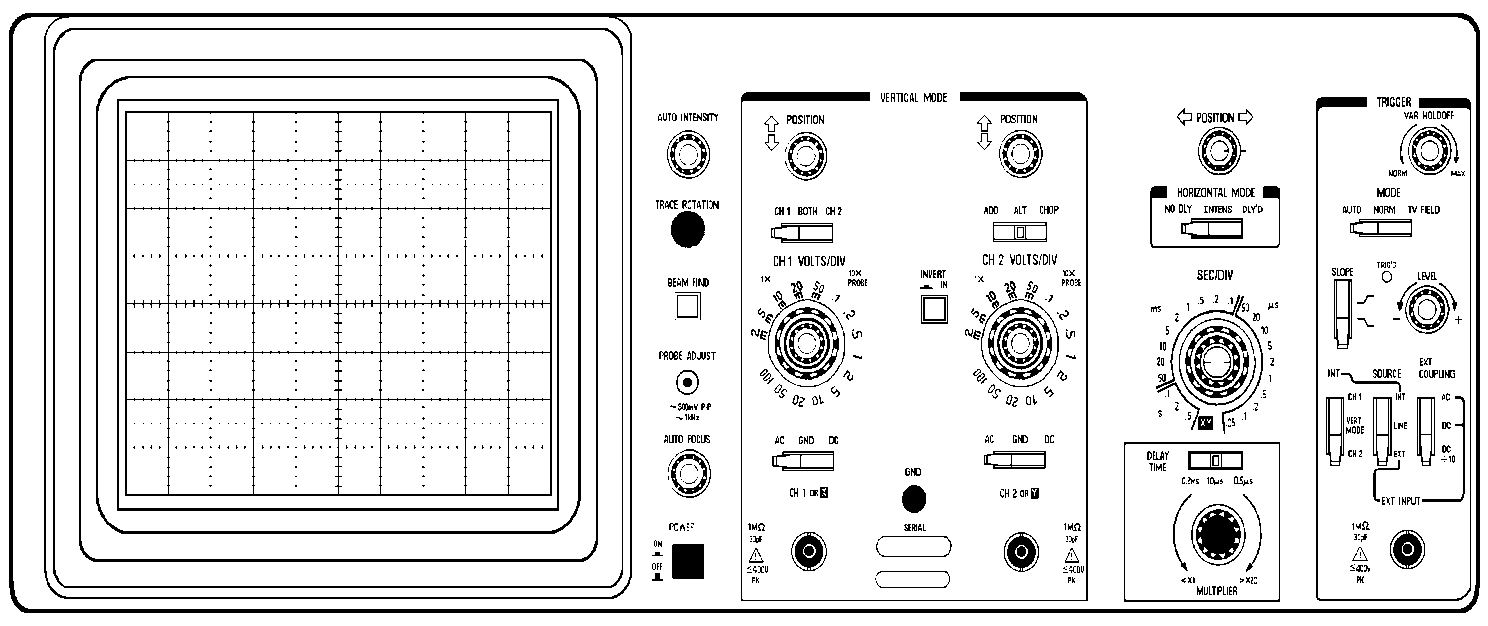
\includegraphics[width=140pt]{/usr/local/master/labs/physics397-FA2016/RLC-Resonant-Circuits/RLC-Resonant-Circuits-osc-controls.png}}; %oscillocope
\draw[thick](0,.8)rectangle(.5,1);
\node[shape=circle,draw=black,fill=black,scale=.7] at(0,.9){};
\node[shape=circle,draw=black,fill=black,scale=.7] at(.5,.9){};
\draw[thick](1,.8)rectangle(1.5,1);
\node[shape=circle,draw=black,fill=black,scale=.7] at(1.0,.9){};
\node[shape=circle,draw=black,fill=black,scale=.7] at(1.5,.9){};

%circuit
\draw[ultra thick](1,4.3)--(1,3.5)--(2.75,3.5)--(2.75,0)--(0,0)--(0,.9);
\draw[ultra thick](1,0)--(1,.9);
\draw[ultra thick](2.75,1)--(4,1);
\draw[](4,1)to [ac source](4,4)--(5,4); %ac source
\draw[decorate,decoration={coil,segment length=8,amplitude=5}](5,4)--(6.5,4); %inductor
\draw[](6.5,4)--(7.5,4)to[capacitor](7.5,1)--(6.5,1); %capacitor
\draw[decorate,decoration={zigzag,segment length=7,amplitude=5}](6.5,1)--(5,1); %resistor
\draw[](5,1)--(4,1)--(4,.5);
\node[ground,rotate=-90]at(4,.4){}; %ground
\draw(7.5,1)--(5.5,-.5)--(1.5,-.5)--(1.5,-.4);
\draw(1.5,.4)--(1.5,.8);
\draw(.5,.15)--(.5,.8);
\draw(.5,-.1)--(.5,-.25)--(3,-.25)--(3,.8);
\draw(3,1.2)--(3,4)--(4,4);
\draw[](3,3.75)--(1.5,3.75)--(1.5,4.25);
\draw(.5,-.1)arc(-90:-270:.1 and .12);
\draw(1.5,-.4)arc(-90:-270:.1 and .4);
\draw(3,.8)arc(-90:-270:.1 and .2);
%labels
\node[font=\footnotesize]at(-1,0.25){Channel 1};
\node[font=\footnotesize]at(2.15,0.39){Channel};
\node[font=\footnotesize]at(2.15,0.15){2};
\node[font=\small]at(-.25,0.75){B};
\node[font=\small]at(.75,0.6){RB};
\node[font=\small]at(1.75,0.75){R};
\node[font=\small]at(0,3.25){Oscilloscope};
\node[font=\small]at(0,6){Function Generator};
\node[font=\small]at(.5,4){Black};
\node[font=\small]at(1.85,4){Red};
\node[font=\small]at(3.5,1.25){Black};
\node[font=\small]at(3.5,3.75){Red};
\node[shape=circle,scale=.4,fill=black] at (4,4){};
\node[shape=circle,scale=.4,fill=black] at (4,1){};
\node[shape=circle,scale=.4,fill=black] at (7.5,4){};
\node[shape=circle,scale=.4,fill=black] at (7.5,1){};
\draw[rounded corners=15,->](7,2.5)--(7,1.5)--(6,1.5);
\node[font=\small]at(4.25,1.25){a};
\node[font=\small]at(7.25,1.25){b};
\node[font=\small]at(7.25,3.75){c};
\node[font=\small]at(4.25,3.75){d};
\node[font=\small]at(5.75,.6){R};
\node[font=\small]at(5.75,3.5){L};
\node[font=\small]at(7.75,2.8){C};
\node[font=\small]at(6.5,1.75){$i$};
\end{tikzpicture}
\caption{Series RLC circuit setup.}
\label{fig:rc4}
\end{figure}

\item Find the amplitude/phase resonance by scanning through frequencies near the theoretical value. Stop varying the frequency when the channel 2 trace has its amplitude extremum. Record the experimental resonant frequency from the function generator. Verify that the frequency for amplitude resonance is the same as the frequency for phase resonance ($\phi= 0$).

\item For the resonant frequency and at least 20 other frequencies, some below and some above the resonant frequency, record the peak-to-peak voltage value from the oscilloscope.

\item For the {\bf parallel RLC circuit}, setup the experiment as in Figure \ref{fig:rc5}. Connect both the function generator and channel 1 of the oscilloscope between the red and black input pins (between point {\bf a} and ground). Thus the trace on channel 1 represents the input signal from the function generator. The hidden resistor under the circuit board is a necessity for the output signal to be different from the input signal and to measure the current.

\begin{enumerate}[label=\alph*)]

\item Connect channel 2 of the oscilloscope between {\bf b} and ground. Remember that black lead goes into the black terminal. Also, short out the resistor positioned below the inductor using the shorting wire provided. This is necessary as amplitude resonance is better seen without the resistor since there is less voltage sharing between the inductor and the resistor and the hidden resistor has less effect.

\item Find the amplitude resonance by scanning through frequencies near the theoretical value. Record the experimental resonant frequency from the function generator. 

\item For the resonant frequencies and at least 20 other frequencies, some below and some above the resonant frequencies, record the peak-to-peak voltage value from the oscilloscope.

 \item Remove the shorting wire from the resistor and find the phase resonance. The reason for removing the shorting clip is that the frequency difference between amplitude and phase resonance is magnified for a larger resistance in series with the inductor. There are two common methods for measuring a phase difference. One method was outlined previously. Another technique is to switch the oscilloscope timebase to x-y mode which plots channel 1 versus channel 2 on the screen. When the signals are out of phase a loop appears on the screen. When the two signals are in phase the loop becomes completely closed into a line of positive slope. When the two signals are 180$^{\circ}$ out of phase the loop again closes but this time into a line of negative slope. 

\end{enumerate}
\end{enumerate}

\begin{figure}
\begin{tikzpicture}[circuit ee IEC]
\node at (0,5){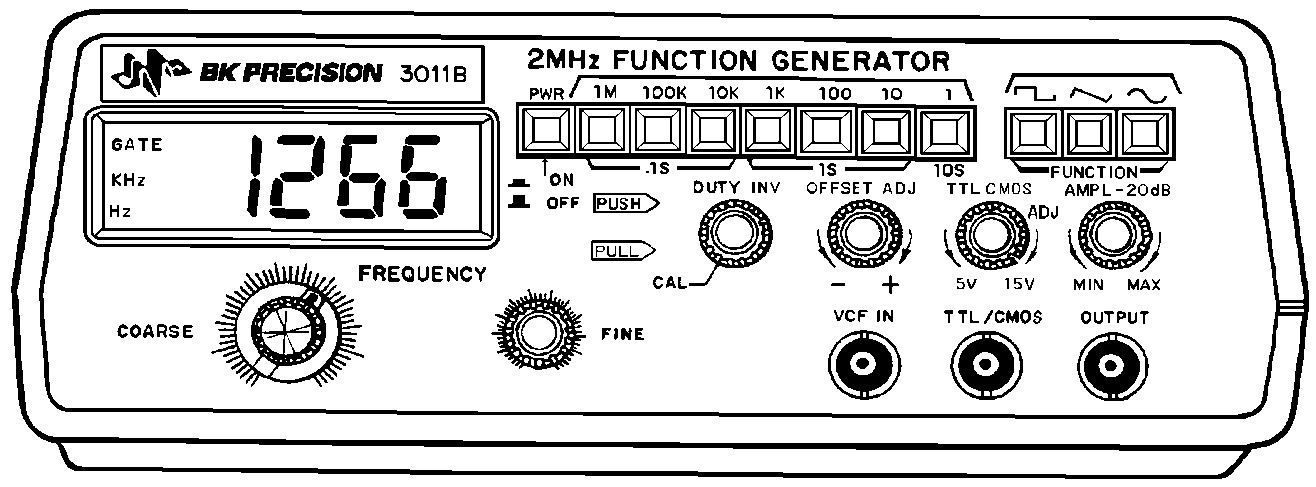
\includegraphics[width=110pt]{/usr/local/master/labs/physics397-FA2016/RLC-Resonant-Circuits/RLC-Resonant-Circuits-func-gen.png}}; %function generator
\draw[thick](1,4.2)rectangle(1.5,4.4);
\node[shape=circle,draw=black,fill=black,scale=.7] at(1.0,4.3){};
\node[shape=circle,draw=black,fill=black,scale=.7] at(1.5,4.3){};
\node at (0,2){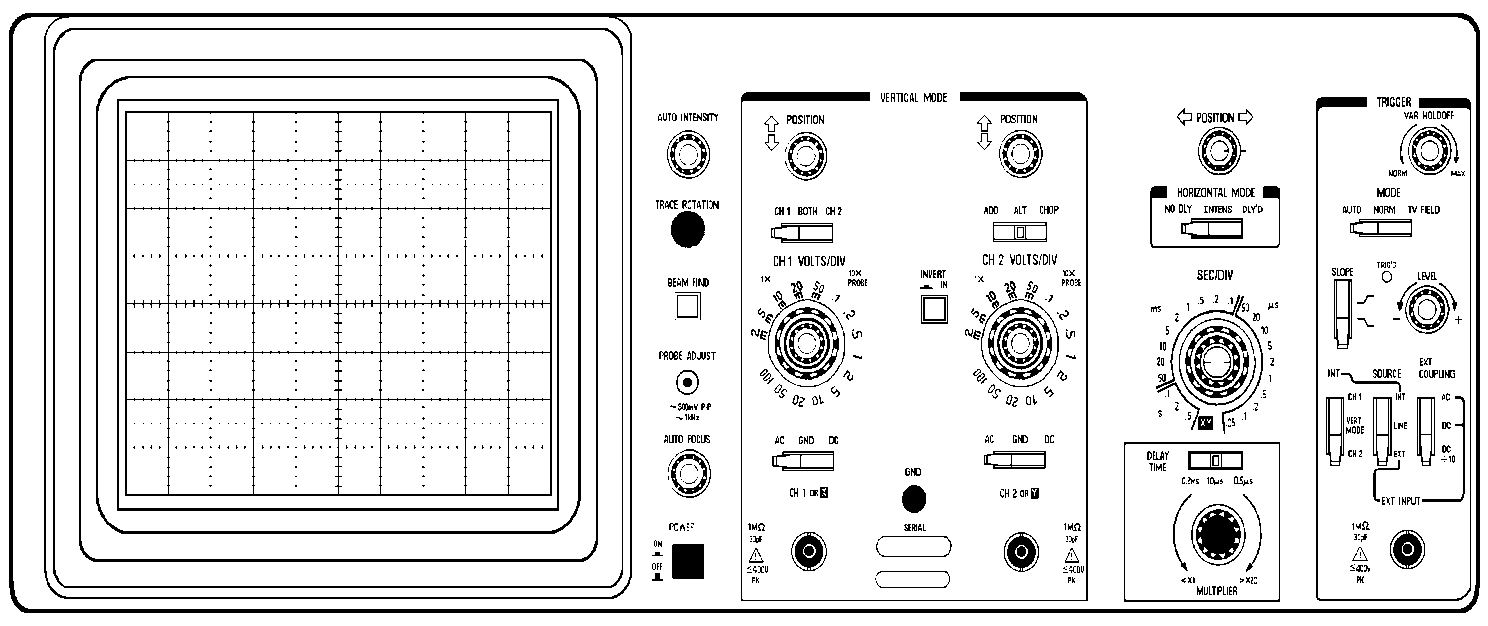
\includegraphics[width=140pt]{/usr/local/master/labs/physics397-FA2016/RLC-Resonant-Circuits/RLC-Resonant-Circuits-osc-controls.png}}; %oscillocope
\draw[thick](0,.8)rectangle(.5,1);
\node[shape=circle,draw=black,fill=black,scale=.7] at(0,.9){};
\node[shape=circle,draw=black,fill=black,scale=.7] at(.5,.9){};
\draw[thick](1,.8)rectangle(1.5,1);
\node[shape=circle,draw=black,fill=black,scale=.7] at(1.0,.9){};
\node[shape=circle,draw=black,fill=black,scale=.7] at(1.5,.9){};
%circuit
\draw[ultra thick](1,4.3)--(1,3.5)--(2.75,3.5)--(2.75,0)--(0,0)--(0,.9);
\draw[ultra thick](1,0)--(1,.9);
\draw[ultra thick](2.75,1)--(4,1);
\draw[](4,1)to [ac source](4,4)--(5.5,4)--(5.5,3.8); %ac source
\draw[decorate,decoration={coil,segment length=6,amplitude=4}](5.5,3.8)--(5.5,2.5); %inductor
\draw[](5.5,4)--(7.5,4)to[capacitor](7.5,2.25)--(7.5,1)--(5.5,1)--(5.5,1.2); %capacitor
\draw[decorate,decoration={zigzag,segment length=8.5,amplitude=4}](5.5,1.2)--(5.5,2.5); %resistor at c
\draw[](4.2,1)--(4,1)--(4,.5);
\draw[decorate,decoration={zigzag,segment length=8.5,amplitude=4}](4.2,1)--(5.3,1); %resistor at b
\draw[](5.3,1)--(5.5,1);
\node[ground,rotate=-90]at(4,.4){}; %ground
\draw(5.5,1)--(4.5,-.5)--(1.5,-.5)--(1.5,-.4);
\draw(1.5,.4)--(1.5,.8);
\draw(.5,.15)--(.5,.8);
\draw(.5,-.1)--(.5,-.25)--(3,-.25)--(3,.8);
\draw(3,1.2)--(3,4)--(4,4);
\draw[](3,3.75)--(1.5,3.75)--(1.5,4.25);
\draw(.5,-.1)arc(-90:-270:.1 and .12);
\draw(1.5,-.4)arc(-90:-270:.1 and .4);
\draw(3,.8)arc(-90:-270:.1 and .2);
%labels
\node[font=\footnotesize]at(-1,0.25){Channel 1};
\node[font=\footnotesize]at(2.15,0.39){Channel};
\node[font=\footnotesize]at(2.15,0.15){2};
\node[font=\small]at(-.25,0.75){B};
\node[font=\small]at(.75,0.6){RB};
\node[font=\small]at(1.75,0.75){R};
\node[font=\small]at(0,3.25){Oscilloscope};
\node[font=\small]at(0,6){Function Generator};
\node[font=\small]at(.5,4){Black};
\node[font=\small]at(1.85,4){Red};
\node[font=\small]at(3.5,1.25){Black};
\node[font=\small]at(3.5,3.75){Red};
\node[shape=circle,scale=.4,fill=black] at (4,4){};
\node[shape=circle,scale=.4,fill=black] at (4,1){};
\node[shape=circle,scale=.4,fill=black] at (5.5,2.5){};
\node[shape=circle,scale=.4,fill=black] at (7.5,2.5){};
\node[shape=circle,scale=.4,fill=black] at (5.5,1){};
\node[font=\small]at(7.25,2.5){d};
\node[font=\small]at(4.25,3.75){a};
\node[font=\small]at(5.5,.7){b};
\node[font=\small]at(5.25,2.5){c};
\node[font=\small]at(5.2,1.75){R};
\node[font=\small]at(5.8,3.2){L};
\node[font=\small]at(7.75,2.8){C};
\draw[->](7.2,2)--(7.2,1.3); %current arrow
\draw[->](5.8,2)--(5.8,1.3); %current arrow
\draw[->](5,1.3)--(4.25,1.3); %current arrow
\node[]at(4.5,1.5){$i_{tot}$};
\node[]at(7,1.75){$i_{1}$};
\node[]at(6,1.75){$i_{2}$};
\end{tikzpicture}
\caption{Parallel RLC circuit setup}
\label{fig:rc5}
\end{figure}

\section{Error Analysis}
The internal resistance of the function generator is ignored in this experiment. Consider all values written on the circuit boards as exact. The error in an oscilloscope measurement is half the resolution of the measurement scale. Remember to record which voltage scale and time scale the oscilloscope is set on when recording data. 

There are two errors associated with the function generator frequency. A {\bf drift error} caused by temperature variations inside the function generator and a {\bf quantization error} which is associated with any digital instrument. The drift error can be estimated by observing variations in the output frequency. While you are making measurements, take note of the maximum and minimum frequency values displayed on the function generator. The difference between the maximum and the minimum value divided by two gives the associated drift error. If the function generator has been on for some time then no drift in frequency values may be observable. In this case, the only error associated with the frequency will be the quantization error. 

The error resulting from the conversion of a frequency to a digital display is called the quantization error. Manufacturers usually give the value of this error as plus or minus one number in the smallest digit of the display. The manual accompanying the B \& K Precision Function Generator lists this value as $\pm$1 count.

Take the error in frequency to be the sum of the drift and quantization errors. If, for example, the frequency fluctuates from 767 to 771 Hz in the course of resonance measurments, then the frequency is recorded as 769 Hz and the associated drift error will be $\pm$2 Hz. To take into account the quantization error, add $\pm$1 of the last digit shown on the function generator. Thus, if the last digit shown on the function generator is a ones digit, then the quantization error is $\pm$1 Hz. Therefore, the total error would be $\pm$3 Hz.

\section{To be handed in to your lab instructor}

%%% begin prelab %%%
\section{Prelab}
\begin{enumerate}

\item Explain what resonance is and give four examples from physical systems.

\item For the series RLC circuit, derive $\omega^2 = 1/LC$ from Equations \ref{equ:rc7} and \ref{equ:rc8} with the condition that $\phi = 0$. Confirm that phase and amplitude resonance occur at the same frequency.

\item For the parallel RLC circuit, derive Equation \ref{equ:rc15} from Equation \ref{equ:rc13}.

\item Justify the use of Equations \ref{equ:rc6}, \ref{equ:rc9}, \ref{equ:rc10}, and \ref{equ:rc11} for the particular circuits, series and parallel.

\item Show that when R=0 in the parallel RLC circuit, both the amplitude resonant frequency and the phase resonant frequency are equal and have the same expression as the resonant frequency of the series RLC circuit.
\end{enumerate}
%%% end prelab %%%

\section{{\bf Data Requirements}}
\begin{enumerate}[resume]

\item Calculation of the theoretical amplitude and phase resonance frequencies for both the series and parallel RLC circuits (procedure step 2).

\item Experimental amplitude and phase resonance frequencies, with uncertainties, for both the series and parallel RLC circuits (procedure steps 4, 7, and 9).

\item Table of peak-to-peak voltage measurements from the oscilloscope for at least 20 nonresonant frequencies for the series and parallel RLC circuits (procedure steps 5 and 8).

\item For the series RLC circuit, provide a table with numerical values for $\omega$, f, and V(p-p), and their uncertainties. Remember that function generators give frequency readings not angular frequencies.

\item For the series RLC circuit, plot V (p-p) versus $\omega$.

\item On the same plot, graph the corresponding theoretical curve of $\dfrac{2E\cdot R_r}{\sqrt{R^2+\left(\omega L-\dfrac{1}{\omega C}\right)^2}}$ versus $\omega$.

\item For the parallel RLC circuit, provide a table with numerical values for $\omega$, f and V (p-p), and their uncertainties.

\item For the parallel RLC circuit, plot V (p-p) versus $\omega$.

\section{Discussion}
\item Compare the theoretical resonant frequencies for both series and parallel RLC circuits with the measured values. Discuss possible sources of error.

\item Comment on the V(p-p) versus $\omega$ plot of the series circuit. Indicate the theoretical and the experimental curves. Also, indicate the corresponding frequency extremum point(s) on your graph. Comment on how well your theoretical curves match the experimental points.

 \item Do your results confirm or refute the theory of resonance? At resonance, is $i$ at its extremum? Justify your conclusion with reference to your results. Consider uncertainties and errors involved in this experiment if you feel that they played significant role in obtaining your conclusion.

\end{enumerate}

\AtEndDocument{\clearpage\ifodd\value{page}\else\null\clearpage\fi} % forces even page count, for double siding

%%%%%%%%%%%%%%%%%%%%%%%%%%%%%%%%%%%%%%%%%%%%%
%
% RLC Resonant Circuits - Companion Guide
%
%%%%%%%%%%%%%%%%%%%%%%%%%%%%%%%%%%%%%%%%%%%%%


\chapter{RLC Resonant Circuits - Companion Guide}

\section{Equipment}
%first column
\begin{minipage}[t]{0.6\textwidth}
\begin{itemize}[noitemsep]
\item Series and parallel RLC circuit board
\item B \& K 3011 function generator
\item set of connecting leads (2)
\end{itemize}
\end{minipage}
%second column
\begin{minipage}[t]{0.35\textwidth}
\begin{itemize}[noitemsep]
\item Oscilloscope
\end{itemize}
\end{minipage}


\section{Setup}
\begin{figure}
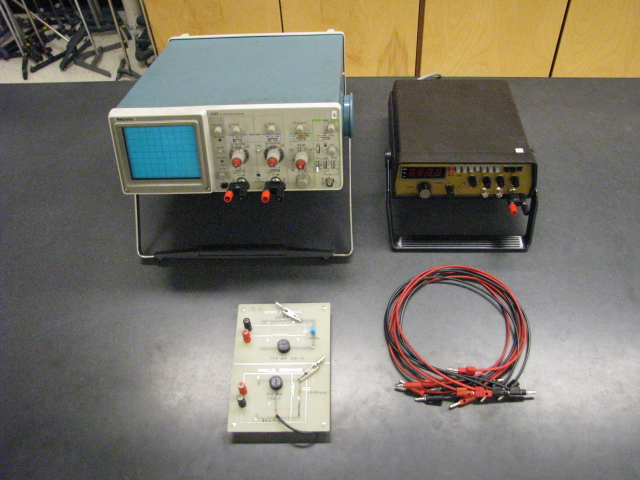
\includegraphics{/usr/local/master/labs/physics397-FA2016/RLC-Resonant-Circuits/RLC-Resonant-Circuits-Setup.jpg}
\caption{Equipment Setup}
\label{pic:RLCsetup}
\end{figure}

Set up bench as shown in Figure \ref{pic:RLCsetup}.

\section{Maintenance}

\begin{enumerate}
\item 
\item 
\end{enumerate}

\section{Critical Points of Failure}

There are currently no known critical points of failure.

\section{Notes to the Instructor}
\begin{enumerate}
\item The function generator outputs a dip on each node for the parallel circuit at amplitude resonant frequency. This caused difficulty in measuring the experimental amplitude resonant frequency since the output frequency could be adjusted within a 100 Hz range while still exhibiting resonant attributes on the oscilloscope. 
\item 
\item 
\end{enumerate}

\section{Prelab Questions}
\begin{enumerate}
\item Resonance is the tendency of a system to oscillate with a greater amplitude at some frequencies than at others (Wikipedia - Resonance). Four examples of physical systems that exhibit resonant qualities: musical instruments (acoustic resonance), suspension systems (mechanical resonance), electrical circuits (electrical resonance), and optical cavities (optical resonance).
\item Derivation of $\omega^2 = 1/LC$: First set $\phi=0$ in Equation 8 (the condition for phase resonance),
$$
0=tan^{-1}\left[ \frac{1}{R} \left( \omega L - \frac{1}{\omega C} \right) \right]
$$
Rearrange to get,
$$
\omega L - \frac{1}{\omega C} =0
$$
Yielding,
$$
\omega^2 = \frac{1}{LC}
$$

Then we can see that Equation 7 is at an extremum (condition for amplitude resonance) when $\omega^2 = \frac{1}{LC}$ giving
$$
E\sin\omega t = i(t)R
$$
which is the maximal current possible for the circuit. Therefore, amplitude resonance and phase resonance occur at the same frequency $\omega=1/\sqrt{LC}$.
\item Parallel phase frequency derivation: First set $\phi=0$ in Equation 13 (the condition for phase resonance) and factor $\omega$ out to get,
$$
\omega\left[\frac{\omega^2L^2C}{R}+RC-\frac{L}{R}\right]=0
$$
Rearrange to get Equation 15,
$$
\omega_P^2 = \frac{1}{LC} -\frac{R^2}{L^2}
$$
\item Justification for Equation 6 (series circuit): Substituting voltage values into Equation 1 we have,
$$
L\frac{di}{dt}+\frac{Q}{C}+iR-E\sin\omega t = 0
$$
Taking the derivative of this gives,
$$
L\frac{d^2i}{dt^2} + R\frac{di}{dt} + \frac{i}{C} - E\omega\cos\omega t = 0
$$

which is Equation 6 from the lab manual. Therefore, this equation is valid to use for a series circuit.

Justification for Equations 9, 10, and 11 (parallel circuit): Equation 9 comes from the current splitting at the node (Kirchhoff's current law) that can be seen in Figure 4. We can then treat each current, $i_1$ and $i_2$, as part of a separate circuit. Equation 10 corresponds to $i_1$ where the voltage source, inductor, and resistor are seen as one circuit. Then Kirchhoff's voltage law is applied to give Equation 10. Equation 11 corresponds to $i_2$ in the same way where just the capacitor and voltage sources are seen as the second circuit. Kirchhoff's voltage law is applied to the circuit and then the derivative is taken with respect to time to give Equation 11.
\item Setting R=0 in Equation 14 gives,
$$
\omega_A ^2 = \frac{1}{LC}
$$
Similarly for Equation 15,
$$
\omega_P ^2 = \frac{1}{LC}
$$
which implies that 
$$
\omega_A=\omega_P=\omega=\frac{1}{\sqrt{LC}}
$$
So, the resonant frequencies in the parallel circuit are equal when there is no resistance and are also equal to the resonant frequency of the series circuit.
\end{enumerate}


\section{Data Requirements}
\begin{enumerate}[resume]
\item The series circuit values were recorded to be: R=50.8 $\Omega$, C=1.00$\times$10$^{-6}$ F, L=0.474 H. When substituted into,
$$
f=\frac{1}{2\pi\sqrt{LC}}
$$
the theoretical resonant frequency was found to be f=231.17 Hz.

The parallel circuit values were recorded to be: R=3263 $\Omega$, C=9.00$\times$10$^{-9}$ F, L=0.475 H. When substituted into,
$$
f_A=\frac{1}{LC}\sqrt{1+\frac{2R^2C}{L}}-\frac{R^2}{L^2}
$$
and
$$
f_P=\frac{1}{2\pi}\sqrt{\frac{1}{LC}\sqrt{1+\frac{2R^2C}{L}}-\frac{R^2}{L^2}}
$$
the theoretical amplitude resonant frequency was found to be f$_A$=2404.49 Hz and the theoretical phase resonant frequency was found to be f$_P$=2135.10 Hz.
\item The experimental resonant frequency for the series circuit was found to be f=230$\pm$ 2 Hz. For the parallel circuit, the experimental amplitude resonant frequency was found to be f$_A$=2300$\pm$ 20 Hz and the experimental phase resonant frequency was found to be f$_P$=2000$\pm$ 20 Hz.
\item See Data Requirement 9 (asks for the same table)
\newpage
\item Table: Series Voltage vs. Frequency and Angular Frequency
\begin{table}[h]
\center
\begin{tabular}{|c|c|c|c|c|c|}
\hline
f (Hz) & $\Delta$f (Hz) & $\omega$ (rad/s) & $\Delta\omega$ (rad/s) & V (V) & $\Delta$V (V)\\
\hline
158 & 2 & 993  & 10 & 0.34 & 0.05\\
169 & 2 & 1060 & 10 & 0.39 & 0.05\\
180 & 1 & 1130 & 6  & 0.44 & 0.05\\
192 & 2 & 1210 & 10 & 0.5  & 0.05\\
200 & 2 & 1260 & 10 & 0.54 & 0.05\\
211 & 1 & 1330 & 6  & 0.59 & 0.05\\
220 & 2 & 1380 & 10 & 0.62 & 0.05\\
225 & 2 & 1410 & 10 & 0.62 & 0.05\\
230 & 2 & 1450 & 10 & 0.62 & 0.05\\
235 & 2 & 1480 & 10 & 0.62 & 0.05\\
240 & 1 & 1510 & 6  & 0.61 & 0.05\\
245 & 2 & 1540 & 10 & 0.6  & 0.05\\
247 & 1 & 1550 & 6  & 0.59 & 0.05\\
250 & 2 & 1570 & 10 & 0.58 & 0.05\\
258 & 2 & 1620 & 10 & 0.56 & 0.05\\
269 & 1 & 1690 & 6  & 0.52 & 0.05\\
284 & 1 & 1780 & 6  & 0.46 & 0.05\\
295 & 2 & 1850 & 10 & 0.43 & 0.05\\
309 & 1 & 1940 & 6  & 0.39 & 0.05\\
322 & 2 & 2020 & 10 & 0.36 & 0.05\\
\hline
\end{tabular}
\label{tbl:RLCSeries}
\caption{Series Resonant Circuit Data}
\end{table}

\item Graph: Series voltage vs. angular frequency
  \begin{figure}[h!]
    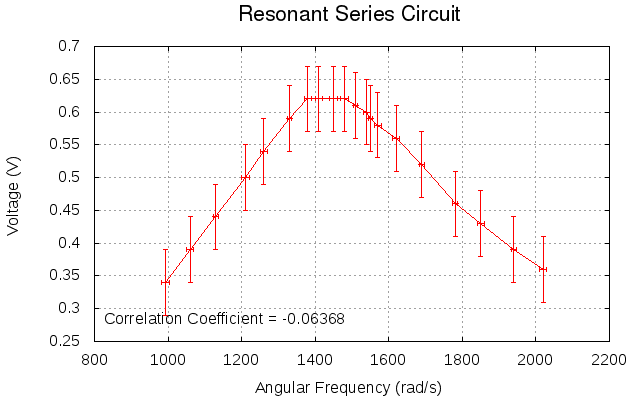
\includegraphics{/usr/local/master/labs/physics397-FA2016/RLC-Resonant-Circuits/RLC-Resonant-Circuits-Series-Graph.png}
    \caption{Resonant Series Circuit}
    \label{pic:RLCseries}
  \end{figure}
\item Graph: Series voltage vs. angular frequency: Experimental vs. Theoretical
  \begin{figure}[h!]
    \center
    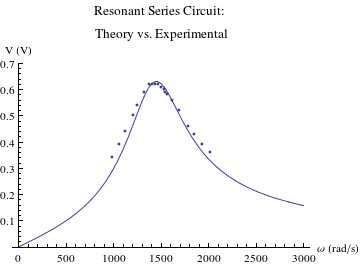
\includegraphics{/usr/local/master/labs/physics397-FA2016/RLC-Resonant-Circuits/RLC-Resonant-Circuits-Series-Graph-Mathematica.png}
    \caption{Resonant Series Circuit: Theoretical vs. Experimental}
    \label{pic:RLCseriesMathematica}
  \end{figure}

\newpage
\item Table: Parallel voltage vs. frequency vs. angular frequency
\begin{table}[h]
\center
\begin{tabular}{|c|c|c|c|c|c|}
\hline
f (kHz) & $\Delta$f (kHz) & $\omega$ (krad/s) & $\Delta\omega$ (krad/s) & V (V) & $\Delta$V (V)\\
\hline
1.50&0.02&9.42&0.13&8.80&1.00\\
1.60&0.01&10.1&0.06&8.00&0.50\\
1.70&0.02&10.7&0.13&7.20&0.50\\
1.80&0.02&11.3&0.13&6.30&0.50\\
1.90&0.02&11.9&0.13&5.30&0.50\\
2.00&0.02&12.6&0.13&4.30&0.50\\
2.10&0.02&13.2&0.13&2.90&0.25\\
2.20&0.02&13.8&0.13&1.75&0.25\\
2.25&0.02&14.1&0.13&1.18&0.10\\
2.30&0.02&14.5&0.13&0.94&0.10\\
2.35&0.02&14.8&0.13&0.92&0.10\\
2.40&0.02&15.1&0.13&1.40&0.10\\
2.50&0.02&15.7&0.13&2.50&0.25\\
2.60&0.02&16.3&0.13&3.50&0.25\\
2.72&0.02&17.1&0.13&4.50&0.50\\
2.80&0.02&17.6&0.13&5.20&0.50\\
2.90&0.02&18.2&0.13&5.90&0.50\\
3.00&0.02&18.8&0.13&6.50&0.50\\
3.10&0.02&19.5&0.13&7.10&0.50\\
3.20&0.02&20.1&0.13&7.50&0.50\\
\hline
\end{tabular}
\label{tbl:RLCParallel}
\caption{Parallel Resonant Circuit Data}
\end{table}
\item Graph: Parallel voltage vs. angular frequency
  \begin{figure}[h!]
    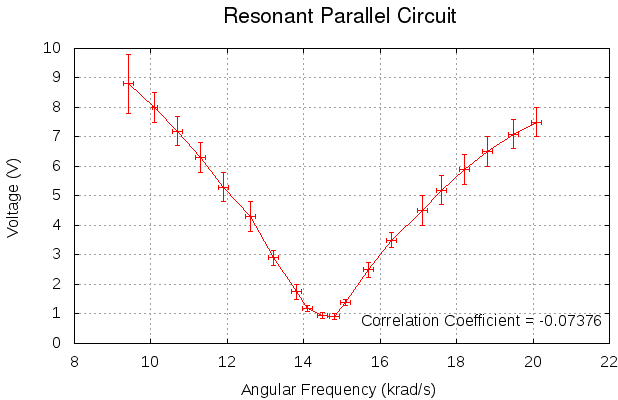
\includegraphics{/usr/local/master/labs/physics397-FA2016/RLC-Resonant-Circuits/RLC-Resonant-Circuits-Parallel-Graph.png}
    \caption{Resonant Parallel Circuit}
    \label{pic:RLCParallel}
  \end{figure}
\end{enumerate}


\section{Discussion}
\begin{enumerate}[resume]
\item The theoretical series resonant frequency was found to be f=231.17 Hz and the experimental value was found to be f=230$\pm$ 2 Hz. These values agree within error. 

For the parallel circuit, the theoretical amplitude resonant frequency was found to be f$_A$=2404.49 Hz and the experimental amplitude resonant frequency was found to be f$_A$=2350$\pm$ 70 Hz where the drift on the function generator occurred from 2300-2400 Hz and was accounted in the error by adding an extra 50 Hz to the original 20 Hz error inherent in the device. The theoretical phase resonant frequency was found to be f$_P$=2135.10 Hz and the experimental phase resonant frequency was found to be f$_P$=2120$\pm$ 20 Hz. Both the phase and amplitude resonant frequencies agreed within error.

Possible sources of error include: degraded devices on the circuit boards, degraded wiring, and the difficulties associated with measuring the theoretical amplitude frequency discussed in the notes below.

\textit{Notes: The function generator output exhibited a dip on each node, which made it difficult to record a proper measurement for the resonant frequencies on the parallel circuit. This error was taken into account for the amplitude resonant frequency measurement as discussed above.}
\item In Figure \ref{pic:RLCseriesMathematica}, the experimental data was plotted along with the theoretical curve. The theoretical extremum point, resonance, occurred at about 6.25 V which corresponded to the experimental resonance at $0.62\pm0.05 V$ within the error range. 
\item The results of this experiment confirm the theory of resonance, as all theoretical values matched experimental within the error range (discussed in Discussion 14).

At resonance, the current was found to be at an extremum for both the series and parallel circuits as predicted by Equations 7 and 12 from the lab manual within the experimental error range. This can be seen when values for angular frequency are substituted into Equations 7 and 12.

\end{enumerate}

\end{document}
